%\documentstyle[epsf,twocolumn]{jarticle}       %LaTeX2.09�d�l
\documentclass[twocolumn]{jarticle} 
%%%%%%%%%%%%%%%%%%%%%%%%%%%%%%%%%%%%%%%%%%%%%%%%%%%%%%%%%%%%%%
%%
%%%%%%%%%%%%%%%%%%%%%%%%%%%%%%%%%%%%%%%%%%%%%%%%%%%%%%%%%%%%%%%%
\setlength{\topmargin}{-45pt}
%\setlength{\oddsidemargin}{0cm} 
\setlength{\oddsidemargin}{-7.5mm}
%\setlength{\evensidemargin}{0cm} 
\setlength{\textheight}{24.1cm}
%setlength{\textheight}{25cm} 
\setlength{\textwidth}{17.4cm}
%\setlength{\textwidth}{172mm} 
\setlength{\columnsep}{11mm}


%�y�߂������邲�Ƃ�(1.1)(1.2) �c(2.1)(2.2)�Ɛ����ԍ����‚����Ƃ��z
%\makeatletter
%\renewcommand{\theequation}{%
%\thesection.\arabic{equation}} %\@addtoreset{equation}{section}
%\makeatother

%\renewcommand{\arraystretch}{0.95} �sT�̐ݒ�

%%%%%%%%%%%%%%%%%%%%%%%%%%%%%%%%%%%%%%%%%%%%%%%%%%%%%%%%
\usepackage[dvipdfmx]{graphicx}  %pLaTeX2e�d�l(�v\documentstyle ->\documentclass)
\usepackage{bm}
\usepackage{amsmath, amssymb}
\usepackage{enumerate}
\usepackage{listings}    %ソースコード入れる用
%%%%%%%%%%%%%%%%%%%%%%%%%%%%%%%%%%%%%%%%%%%%%%%%%%%%%%%%
%ここからソースコードの表示に関する設定
\lstset{
  basicstyle={\ttfamily},
  identifierstyle={\small},
  commentstyle={\smallitshape},
  keywordstyle={\small\bfseries},
  ndkeywordstyle={\small},
  stringstyle={\small\ttfamily},
  frame={tb},
  breaklines=true,
  columns=[l]{fullflexible},
  numbers=left,
  xrightmargin=0zw,
  xleftmargin=0zw,
  numberstyle={\scriptsize},
  stepnumber=1,
  numbersep=1zw,
  lineskip=-0.5ex
}

\begin{document}

\twocolumn[
\noindent

\hspace{1em}
令和3年6月30日(水) 第2回三菱共同会議資料
\hfill
B4 尾關 拓巳

\vspace{2mm}

\hrule

\begin{center}
{\Large \bf 進捗報告}
\end{center}


\hrule
\vspace{3mm}
]

\section{第2回までにしたこと}
\begin{itemize}
    \item Pyomo の検討
    \item Nelder-Mead法とCMA-ESを用いた最適化
\end{itemize}

\section{問題設定}
ガスタービン一台,ボイラ一台,ターボ式冷凍機一台,蒸気吸収式冷凍機二台の5つの機器からなるエネルギープラントの24時刻運用問題であり,120次元の入力変数 $\bm{x}$ が存在する.表\ref{explain_variables}に $\bm{x}$ の定義域を示す.なお,変数の定義域は各機器が稼働時のものであり,停止時は0となる.
\begin{table}[hbtp]
    \caption{変数説明}
    \label{explain_variables}
    \centering
    \begin{tabular}{|c|c|c|}
        \hline
        変数 & 変数の定義域 & 変数の意味 \\
        \hline
        $x_t$ & 1.5〜5.0 & ターボ式冷凍機の熱生成量 \\
        $x_{s1}$ & 4.5〜15.0 & 蒸気吸収式冷凍機1の熱生成量 \\
        $x_{s2}$ & 4.5〜15.0 & 蒸気吸収式冷凍機2の熱生成量 \\
        $x_g$ & 1103〜3679 & ガスタービンのガス消費量 \\
        $x_b$ & 8.02〜803 & ボイラーのガス消費量 \\
        \hline
    \end{tabular}
  \end{table}

\section{Pyomo の検討}
数理計画法からのアプローチとしていくつかのソルバを検討した.その中でPythonベースのオープンソースの最適化モデリング言語として Pyomo\cite{bynum2021pyomo}\cite{hart2011pyomo}があるため,第一段階として使用することを検討した.Pyomo は多様な最適化機能を備えている.
    \subsection{MindtPy}
    MindtPy(Mixed-Integer Nonlinear Dicomposition Toolbox for Pyomo)\cite{BERNAL2018895}はPyomo で開発されたソフトウェアフレームワークで,分解アルゴリズムを用いて MINLP を解くことができる.MINLP の分解アルゴリズムは,基本的に混合整数線形計画法(MILP)や非線形計画法(NLP)に依存している.MindtPy は Outer Approximation(OA)アルゴリズム\cite{OA}と Extended Cutting Plane(ECP)アルゴリズムが実装されている.

    \subsection{変数・制約条件の多さによるエラー}
    PyomoでMindtPyを用いてベンチマーク問題の実装をし,実行した結果,エラーが発生した.Listing \ref{error}にそのエラーを示す.
    \begin{lstlisting}[caption = 発生したエラー, label = error]
        ValueError: MindtPy unable to handle relaxed NLP termination condition of other. Solver message: Too few degrees of freedom (rethrown)!
    \end{lstlisting}
   このエラーは MindtPy の非線形計画問題(NLP)部分のソルバーとして使われているInterior Point Optimizer(Ipopt)で発生し,制約条件や変数が多すぎることを意味する.メモリーが多いサーバでの実行,変数の固定をしたが結果は変わらなかった.一方で,最適化する運用時刻数を小さくし,定義する変数や制約条件自体を減らすと実行できた.
  
\section{Nelder-Mead 法と CMA-ESを用いた最適化}
エネルギープラント運用計画のための最適化ベンチマーク問題 ver.1\cite{denki}を対象とする.なお,deapのcmaのStrategyを使用した.\cite{DEAP_JMLR2012}

単目的最適化の場合(Strategy)は元の目的関数を $f$, 機器の上下限制約,起動・停止状態などの満たすべき等式・不等式をまとめた制約違反関数を $V$, ペナルティ関数の重みを $\rho$ とすると, Nelder-Mead 法及び CMA-ES 上での目的関数 $F$ は(\ref{F})式で表される.
\begin{equation}
    \label{F}
    F = f + \rho V
\end{equation}
今回の実験では,制約違反関数 $V$ が $1.0 \times 10^{-10}$ より小さい解を実行可能解と定義する.

予備実験により,Nelder-Mead 法はそのまま適用しても $F$ を十分に小さくできないことがわかったため,決定変数の一部である $\bm{x}$ を固定し,2値で各機器の稼働状態を表す $\bm{y}$ のみの探索をした.$x_i(i=0,1,\dots,120$ は $y_i=0$ ,すなわち機器が停止状態のときは0, そうでないときは各上下限値の平均値とした.そして,Nelder-Mead 法で見つかった最後の解を CMA-ES の初期平均ベクトルとし,初期個体群に加えた.

Nelder-Mead 法では各値が離散値である $\bm{y}$ を連続変数で探索できるように,最初の単体における頂点座標の各値を0.99以上1.01以下のランダムな実数と設定して探索し,目的関数内で各値が1より小さければ0, そうでないとき1,と処理した後に評価した.

CMA-ES では $f$ が定めた閾値 $t$ より小さくなったら $F$ にペナルティを与えることで,$\rho$ を小さくしても探索中に目的関数が小さくなりすぎて実行不可能な領域を探索することを防いだ.

\section{実験}
表\ref{setting_nelder}にNelder-Mead 法で用いた実験パラメータを,表\ref{setting_cmaes}に CMA-ES で用いた実験パラメータを示す.閾値 $t$ は, Nelder-Mead 法により $\{f, V\}=\{3999381.510, 99.58317874\}$ が得られ,実行可能解の $f$ がこの付近の値となると予測したことから決定した.
\begin{table}[htbp]
    \begin{center}
        \caption{Nelder-Mead 法の実験パラメータ}
        \label{setting_nelder}
        \begin{tabular}{| c | c |} \hline
            パラメータ & 値 \\ \hline
            変化とみなす最小変化量 & $1.0\times10^{-5}$ \\
            変化しない場合終了するステップ数 & 200 \\
            最大試行数 & 1000 \\
            $\rho$ (ペナルティ関数の係数) & $1.0\times10^{3}$\\ \hline
        \end{tabular}
    \end{center}
\end{table}

\begin{table}[htbp]
    \begin{center}
        \caption{CMA-ES の実験パラメータ}
        \label{setting_cmaes}
        \begin{tabular}{| c | c |} 
            \hline
            パラメータ & 値 \\ 
            \hline
            $\sigma$ (初期標準偏差) &  0.1 \\
            世代数 & 5000 \\
            入力変数の次元 & 120 \\
            一世代の個体数$\lambda$ & 1200 \\
            $\rho$ (ペナルティ関数の係数) & $1.0\times10^{4}$\\
            $t$ (閾値) & 3999000 \\
            \hline
        \end{tabular}
    \end{center}
\end{table}

表\ref{result}に実験で得た最終的な目的関数値 $f$, 制約違反関数 $V$および既知解を示す.
\begin{table}[htbp]
    \begin{center}
        \caption{実験結果}
        \label{result}
        \begin{tabular}{|c|c|c|}
            \hline
            解法 & 目的関数値 & 制約違反関数 \\ 
            既知解1 & 3999631.278 & $2.44 \times 10^{-10}$ \\
            既知解2 & 3999635.845 & $6.43 \times 10^{-12}$ \\
            既知解3 & 4052185.662 & $3.93 \times 10^{-14}$ \\
            実験    & 4033408.653 & $9.78 \times 10^{-11}$ \\
            \hline
        \end{tabular}
    \end{center}
\end{table}
結果として既知解3より目的関数値が小さい実行可能解を得ることができた.

次に,図\ref{img_F}に最適化をした目的関数 $F$ の推移を,図\ref{img_f}に元の目的関数 $f$ の推移を,図\ref{img_V}に制約違反関数 $V$ の推移を示す.縦軸はそれぞれ $F, f, V$, 横軸は Nelder-Mead 法の試行数と CMA-ES の世代数である.
\begin{figure}
    \centering
    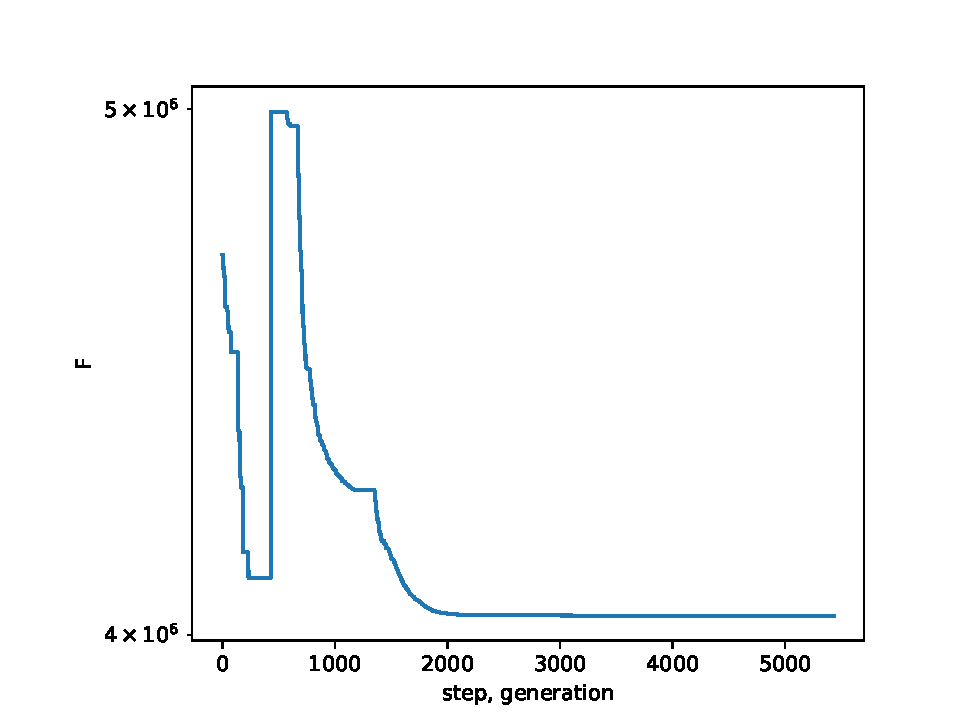
\includegraphics[width=9cm]{img_F.pdf}
    \caption{目的関数値 $F$ の推移}
    \label{img_F}
\end{figure}
\begin{figure}
    \centering
    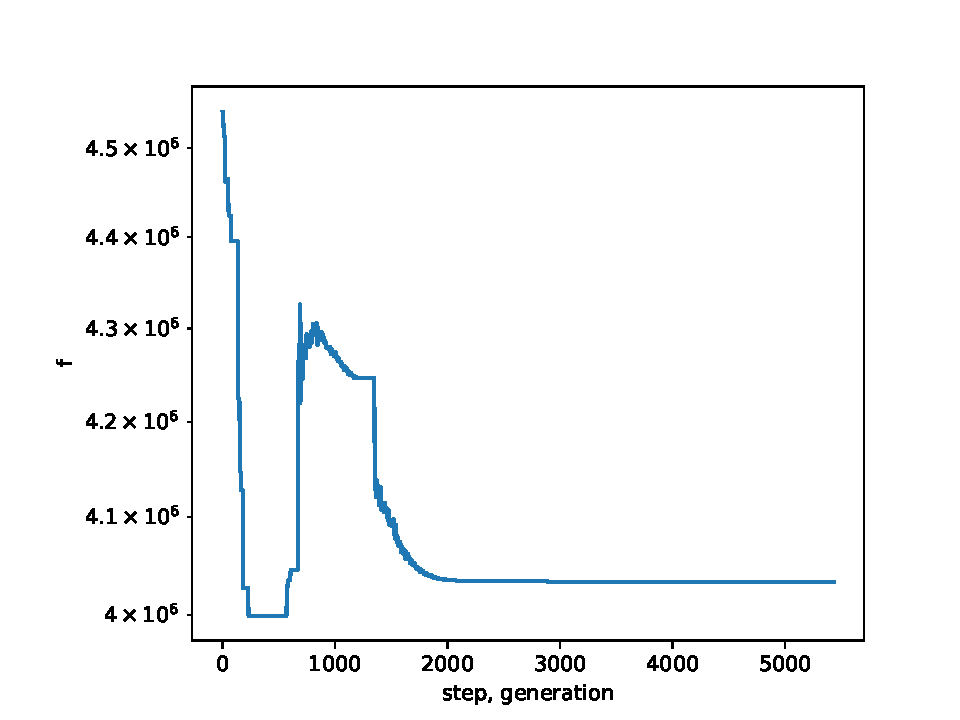
\includegraphics[width=9cm]{img_f.pdf}
    \caption{目的関数値 $f$ の推移}
    \label{img_f}
\end{figure}
\begin{figure}
    \centering
    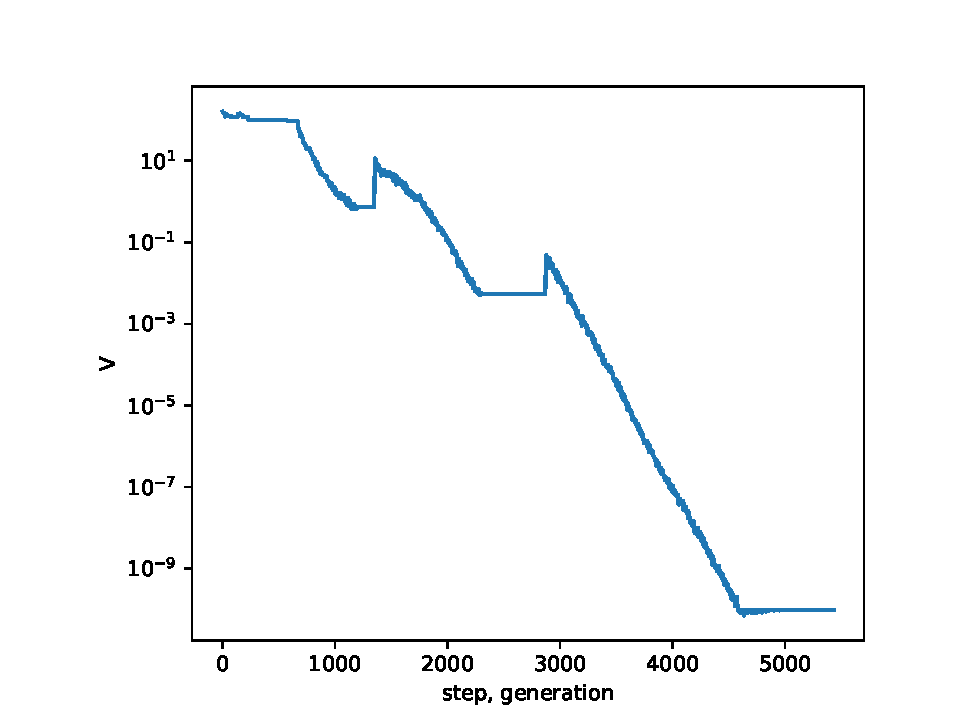
\includegraphics[width=9cm]{img_V.pdf}
    \caption{制約違反関数 $V$ の推移}
    \label{img_V}
\end{figure}
ペナルティ関数の係数 $\rho$ が2手法間で異なり,Nelder-Mead 法は430試行であったため,その前後で $F$ が急に増加している.$f$ は Nelder-Mead 法で400万ほどまで小さくできたが,その後のCMA-ESで一度430万程度まで増加した.また,そのときの $V$ は減少傾向にある.これは  $\rho$ が大きく, $V$ を小さくすることを優先したためだと考えられる.Nelder-Mead 法では, $V$ は最初から低く,あまり減少していない.これは $\bm{x}$ を適切な値に固定したためだと考えた.

\section{今後の展望}
数理計画法からのアプローチで,Pyomo以外のソルバを調査し,検討したい.
また,今回 Nelder-Mead 法と CMA-ES による電力プラントの最適化について検討し,既知解に近い実行可能解を得ることができたが,最良の既知解を改善することはできなかった.今後の課題として,ペナルティ関数の係数を最適化の途中で調整することや,各手法の実験パラメータの調整があげられる.

%参考文献
\bibliographystyle{junsrt}
\bibliography{hoge} %ファイル名

\end{document}